Consider a more practical approach that takes all the previously discussed aspects.
Applying modern frameworks like ASP .NET Core, Angular etc.
let be the following authentication flow as per diagram below
\begin{figure}[H]
    \centering
    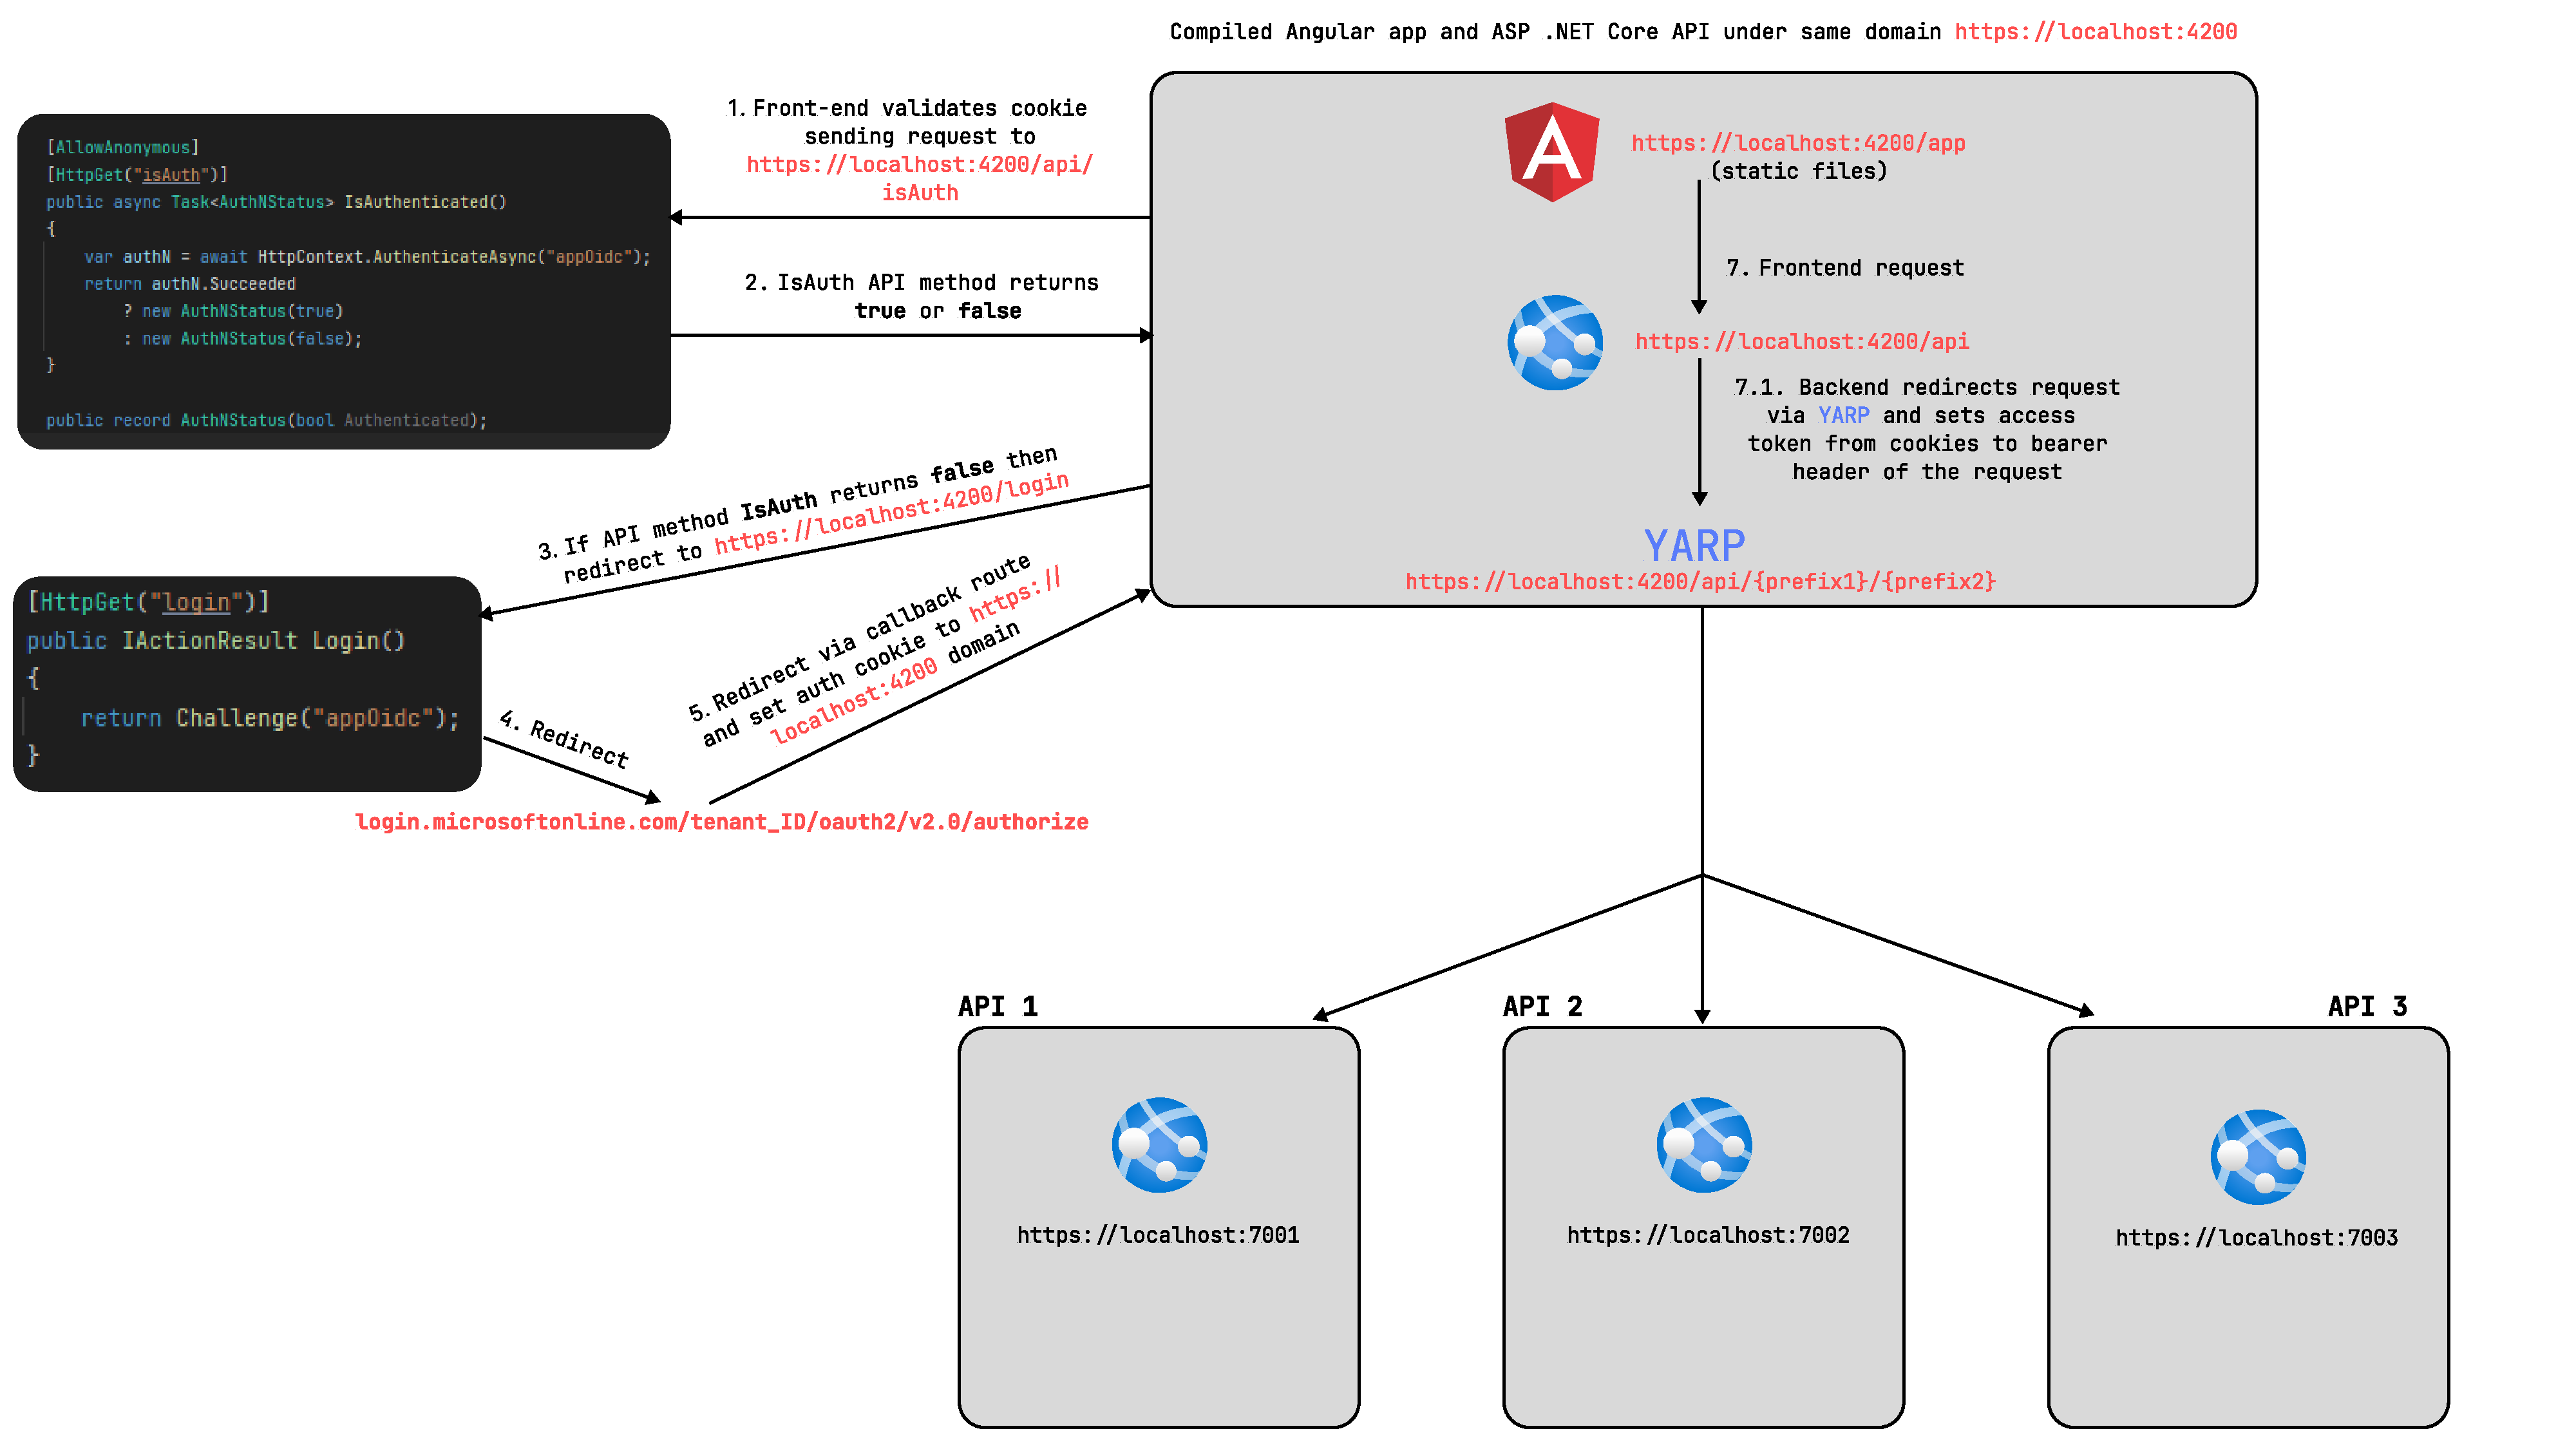
\includegraphics[width=1\textwidth]{img/Auth_flow_updated}
    ~\caption{Authentication flow diagram.}\label{fig:authentication_flow_diagram}
\end{figure}

Therefore, the whole authentication process can be described as nine steps such that
\begin{enumerate}
    \item Compiled Angular frontend application sends request to the authentication endpoint of the ASP .NET Core API
    to verify current authentication state.
    Angular application is a set of precompiled bundles that are exposed via same ASP .NET Core API at the \texttt{/app}
    endpoint so that cross-origin requests are not necessary and tokens can be stored in cookie files securely
    \item Authentication endpoint of the ASP .NET Core API responses either with
    HTTP status code \texttt{200 (OK)} or \texttt{401 (Unauthorized)}
    \item If \texttt{401 (Unauthorized)} status code received from previous step,
    then browser is redirected to the \texttt{login} endpoint of the ASP .NET Core API,
    otherwise user gets access to the protected resources
    \item Login method of the ASP .NET Core API redirects browser to the Azure AD authorize url
    \texttt{login.microsoftonline.com/tenant/oauth2/v2.0/authorize} where user enters his credentials
    \item After successful login on the Azure AD side, the browser is redirected to the \texttt{fallback\_url}
    that is defined in Azure AD application registration.
    This \texttt{fallback\_url} is an active endpoint of the ASP .NET Core API.
    Authentication cookies are being setup at this step.
    \item Step 1 is repeated here, but now the HTTP request is for sure to be with \texttt{200 (OK)} status code.
    \item Precompiled Angular frontend application now sends request to the another microservice with authentication cookies
    attached to the request's \texttt{Bearer} header using YARP library, so that microservice is accessible.
    \item If previous step returns \texttt{401 (Unauthorized)} status code, then Step 1 is repeated
\end{enumerate}